% id: 206-427
% book: 개념원리 기하 · 25 벡터의 내적과 두 벡터가 이루는 각
% section: 필수·발전 예제
% figure: crop:fig-206-427.png
% answer: $\dfrac{3\sqrt{2}}{2}$
% answer_source: 답지
% variant_level: 0 (원본 전사)
% 이 파일은 build.mjs 가 items.json 에서 만든다. 고칠 때는 items.json 을 고친다.
\smash{\raisebox{1.5mm}{\dmkichul{개념원리 기하 206쪽 427번 · 확인체크}}}
\noindent\begin{minipage}[t]{0.58\linewidth}\vspace{0pt}\raggedright 오른쪽 그림의 삼각형~$\pt{OAB}$에서 $|\overrightarrow{\pt{OA}}|=3$, $|\overrightarrow{\pt{OB}}|=2$, $\overrightarrow{\pt{OA}}\cdot\overrightarrow{\pt{OB}}=3\sqrt{2}$일 때, 삼각형~$\pt{OAB}$의 넓이를 구하시오.\end{minipage}\hfill\begin{minipage}[t]{0.4\linewidth}\vspace{0pt}\centering \setlength{\dmfigw}{96.0pt}\ifdim\dmfigw>\linewidth\setlength{\dmfigw}{\linewidth}\fi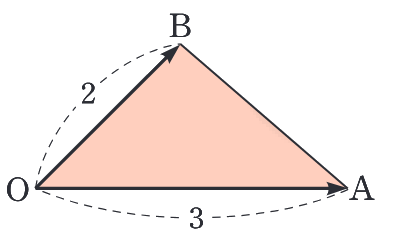
\includegraphics[width=\dmfigw]{figures/fig-206-427.png}\end{minipage}\par
